\subsubsection{The Fundamental Theorem of Linear Algebra}

In order to proof the pending \cref{thm:SVD2} from previous
section, we need to present the four subspaces that an arbitrary
matrix $A$ introduces. But before that, a few important
definitions and remarks: \\

\begin{itemize}
    \item Matrix application $A\vec{x}$ can be seen as a linear
      combination of the columns of $A$:
      \[
      A\vec{x} = 
      \begin{bmatrix}
        \vec{A_1} \mid \vec{A_2} \mid \cdots \mid \vec{A_n}
      \end{bmatrix} \vec{x} = 
      \sum_{i=1}^n x_i \vec{A_i}
      \]
  \item Subspace: A subset of a vector space, which is itself a
    vector space (that is, contains the \vec{0} and is closed under
    the addition and multiplication by an scalar). 
  \item Dimension: Is the size of any basis of a vector space (an
    important result in Linear Algebra, shows that all the basis must
    have the same number of elements; hence, the dimension is a property of the
    space itself). The dimension of a vector space (or subspace) $V$
    is denoted as $\dim{V}$.
  \item Given vector space $V$ and a subspace $W \subset V$ , the
    subspace $\ortc{W} \subset V$ consists of all
    the vectors of $V$ which are orthogonal to all the vectors of
    $W$. $\ortc{W}$ is called the orthogonal complement of $W$.
\end{itemize}
\hfill

Now is right time to talk about the subspaces: we already established
that each matrix of $m \times n$, can be seen as the operational
representation of a linear transformation with signature $\R{n}
\fromto \R{m}$. The action of $A$, in transforming the vectors from
one space to the other, has an interesting effect on each side: both
domain (\R{n}) and codomain (\R{m}), are broken in two orthogonal
pieces. Those pieces actually, happen to be subspaces and their basis
are contained on the matrices $V$ and $U$ of the SVD factorization! But
let us explain piece by piece; a good start, is the column space. \\

The column space of a matrix $A$, is pretty much the concept of the
image of a function; that is, the set of all vectors in 
$A\vec{x} \in \R{m} \suchthat \vec{x} \in \R{n}$, and it is denoted as
$\C{A}$. Another way of looking at it (per one of the remarks above),
is that each application 
of the linear transformation $A$ (that is, each $A\vec{x}$), converts
the input vector \vec{x} into a linear combination of the columns of
A; therefore, $\C{A}$ is the spanning set generated by the
columns of $A$. It can be proved that this subset is actually a
subspace of \R{m}. \\

The next subspace is also clearly understood, is the so called
null space of $A$. It consists of all the solutions to the homogeneous
system $A\vec{x} = \vec{0}$ and is denoted as $\N{A}$. In the
language of transformations, is the set 
of all vectors $\vec{x} \in \R{n}$ that function $A$ compresses into the zero
vector of \R{m}. This subset at least contains the vector \vec{0}, but
in general it will contain much more vectors (only the non-singular
matrices have $\N{A} = \{\vec{0}\}$). Again, it can be proved
that this subset is also a subspace (though this one belongs to \R{n}). \\

The next two subspaces, are not that intuitive to introduce; unless we
think now in terms of the transformation represented by matrix
\trans{A}. This matrix represents a linear transformation that goes
into the opposite direction of $A$, that is, from \R{m} to \R{n}. If
we think in the image of this function $\{\trans{A}\vec{y} \in \R{n} \mid
y \in \R{m} \}$, an interesting realization comes to the picture: what if we
apply the same idea as before, that $\trans{A}\vec{y}$ is a linear
combination of the columns of $\trans{A}$: \\

\[
\trans{A}\vec{y} = 
\begin{bmatrix}
  \vec{(\trans{A})_1} \mid \vec{(\trans{A})_2} \mid \cdots \mid \vec{(\trans{A})_m}
\end{bmatrix} \vec{y} = 
\sum_{i=1}^m y_i \vec{(\trans{A})_i} = 
\sum_{i=1}^m y_i (\text{row $i$ of $A$})
\]
\hfill

In order words, columns of \trans{A} are the rows of $A$, therefore;
the column space of \trans{A} is precisely the row space of original
matrix $A$; this is denoted as \C{\trans{A}} and it can also
be proved that it is a subspace of \R{m}. The last and fourth
subspace, comes from considering the null space of \trans{A}; that is,
those vectors \vec{y} in \R{m} which are compressed into the zero
vector of \R{n}. Is not hard to prove that this is a subspace as
well; it is called the left null space of $A$, and denoted as
\N{\trans{A}}. \\

Summarizing, the four subspaces associated to any
matrix $A$ of $m \times n$ are the following (intuitive proofs that
all of them are indeed subspaces can be found in \cite{strang88}): \\

\begin{itemize}
\item \C{\trans{A}}: row space, lives in \R{n}
\item \N{A}: null space, lives in \R{n}
\item \C{A}: column space, lives in \R{m}
\item \N{\trans{A}}: left null space, lives in \R{m}
\end{itemize}
\hfill

The first thing we note is the intentional grouping of these subspaces;
while \C{\trans{A}} and \N{A} belong to \R{n} [the domain of $A$],
\C{A} and \N{\trans{A}} belong to \R{m} [the codomain of $A$]. These
pairs of subspaces have more in common than merely sharing same
hosting space, they are orthogonal with each other! This is the time
to meet what Strang calls the Fundamental Theorem of Linear Algebra
(part II\footnote{Strang presents the theorem parts in the opposite order
  in \cite{strang88};
  but we preferred to keep our own order, aiming to match better the
  flow of deductions presented in this work.}): \\

\begin{theorem}[Fundamental Theorem of Linear Algebra (part II)]
\label{thm:Fund1}
Let $A$ be a real matrix of $n \times m$, then 

\[
\C{\trans{A}} = \ortc{\N{A}} \ds{\land} \C{A} = \ortc{\N{\trans{A}}}
\]
\end{theorem}
\hfill

\begin{proof}
Let $\vec{x} \in \N{A}$, then \vec{x} satisfies the equation $A\vec{x}
= \vec{0}$; but the resulting vector in \R{m} has as entries the dot product
of \vec{x} with the rows $r_i$ of $A$, therefore, the equation $A\vec{x} =
\vec{0}$ can be rewritten as $m$ equations of the form:

\[
r_i \cdot \vec{x} = 0, \ds{for } 1 \le i \le m
\]

which is essentially saying that the vector \vec{x} is orthogonal to
all the rows $r_i$ of $A$; therefore, it is orthogonal to every linear
combination of them. But those linear combinations are precisely the
row space \C{\trans{A}}; thus $\C{\trans{A}} \perp \N{A}$, or,
reusing previously introduced terminology (see remarks section), we
can say that the row space is the orthogonal complement of the null
space (which is written as $\C{\trans{A}} = \ortc{\N{A}}$).  \\ 

An analogous argument can be constructed for \C{A} and \N{\trans{A}},
using the equation $\trans{A}\vec{y} = \vec{0}$ (details are in
\cite{strang88}). Thus, we can also conclude that the column space is
the orthogonal complement of the left null space (which can be written as $\C{A} =
\ortc{\N{\trans{A}}}$). 
\end{proof}

Having established the orthogonality of these subspaces, allow us to
introduce a secret weapon that will finally help us prove the pending
\cref{thm:SVD2}. This weapon is another theorem that establishes a
relationship between the dimension of any subspace and its orthogonal
complement \footnote{The
  name was provided by us, as Lang does not name it in his book
  \cite{lang04}.}: \\

\begin{theorem}[Orthogonal Complement Dimension Theorem]
\label{thm:ortdim}
Let $W$ any subspace of \R{n}, then is the case that

\[
\dim{W} + \dim{\ortc{W}} = n
\]
\end{theorem}
\hfill

An even more generic version of this theorem is proved by Lang in
\cite{lang04} (theorem 2.3 in that book), and it basically says that
if we take any subspace and its orthogonal complement together, they
form the entirety of the host space! Another way of seeing this
result, is saying that the host space $V$ is the direct sum of the
subspace $W$ and its orthogonal  complement (denoted as $V = W \oplus
\ortc{W}$). Intuitively, the notion 
of a direct sum tells us that there is nothing out of the union of the
subspace $W$ and its orthogonal complement \ortc{W}; every vector in
the original space can be expressed as a sum $x_1 + x_2$ (where
each $\vec{x_1} \in W$ and $\vec{x_2} \in \ortc{W}$, and $W$), and
\ortc{W} do not share anything other than zero vector ($W \cap
\ortc{W} = \{\vec{0}\}$). \\

Using this weapon, we can finally prove the pending 
\cref{thm:SVD2}, which was about proving that the last $n-r$ vectors
of $V$ actually belong to \N{A}. \\

\svdtwo*

\begin{proof}
By hypothesis we know that 

\[
A\vec{v_i} = \sigma_i\vec{u_i}, \ds{}\forall i=1 \dots r, \ds{}\text{where
} r = rank(A).
\]
\\

Since the vectors \vec{u_i}\apos{s} form a basis of \R{m}, that
implies none of them can be zero; therefore $A\vec{v_i} \ne \vec{0}
\ds{}\forall i=1 \dots r$. By definition, such condition implies that
those vectors $v_i \notin \N{A}$, but since $\R{n} = \C{\trans{A}} \oplus \N{A}$,
then the only other option for those vectors
$\{\vec{v_1},\vec{v_2},\dots,\vec{v_r}\}$ is to belong to the row
space \C{\trans{A}}. Actually, since they are all orthogonal, they form
a basis of \C{\trans{A}} (because $\dim{\C{\trans{A}}} = \func{rank}(A) =
r$). Let us call this basis $B_r$. \\

Let $\vec{v_i} \in \R{n}$, which also belongs to
$\{\vec{v_{r+1}},\vec{v_{r+2}},\dots,\vec{v_n}\}$; since \vec{v_i}
is orthogonal to every vector in $B_r$ (as all the \vec{v}\apos{s}
form an orthonormal basis of \R{n}), then \vec{v_i} can not belong
to the subspace generated by $B_r$, which happens to be
\C{\trans{A}}. Using again the fact that $\R{n} = \C{\trans{A}} \oplus
\N{A}$, we can tell that the only other option for $\vec{v_i}$ is to
belong to the nullspace \N{A}. And by definition of nullspace:

\[
A\vec{v_i} = \vec{0}, \ds{}\forall i=(r+1) \dots n
\]
\hfill

which completes the proof. Mirroring the reasoning about basis $B_r$
of the row space, we can also tell that the vectors
$\{\vec{v_{r+1}},\vec{v_{r+2}},\dots,\vec{v_n}\}$ form a basis of the
null space \N{A}. 
\end{proof}

Since we established already the orthogonality between the four
subspaces of matrix $A$, we can simply apply \cref{thm:ortdim}
to them in pairs (depending on whether they are hosted on same space),
and derive the following equations: \\

\begin{enumerate}
\item In \R{n}: $\C{\trans{A}} = \ortc{\N{A}} \implies
  \dim{\N{A}} + \dim{\C{\trans{A}}} = n$
\item In \R{m}: $\C{A} = \ortc{\N{\trans{A}}} \implies 
  \dim{\N{\trans{A}}} + \dim{\C{A}} = m$
\end{enumerate}
\hfill

These two equations are what Strang calls the Fundamental Theorem of
Linear Algebra (Part I); further references are \cite{strang88} and
\cite{strang93}. The two parts of such theorem together, basically
describe what are the subspaces generated by matrix $A$, what is the
relationship among them (orthogonality) and what are their
dimensions. The \cref{fig:fund} below (taken from
\cite{strang88}), summarizes both parts of this important theorem:
\\

\begin{figure}[h]
  \centering
  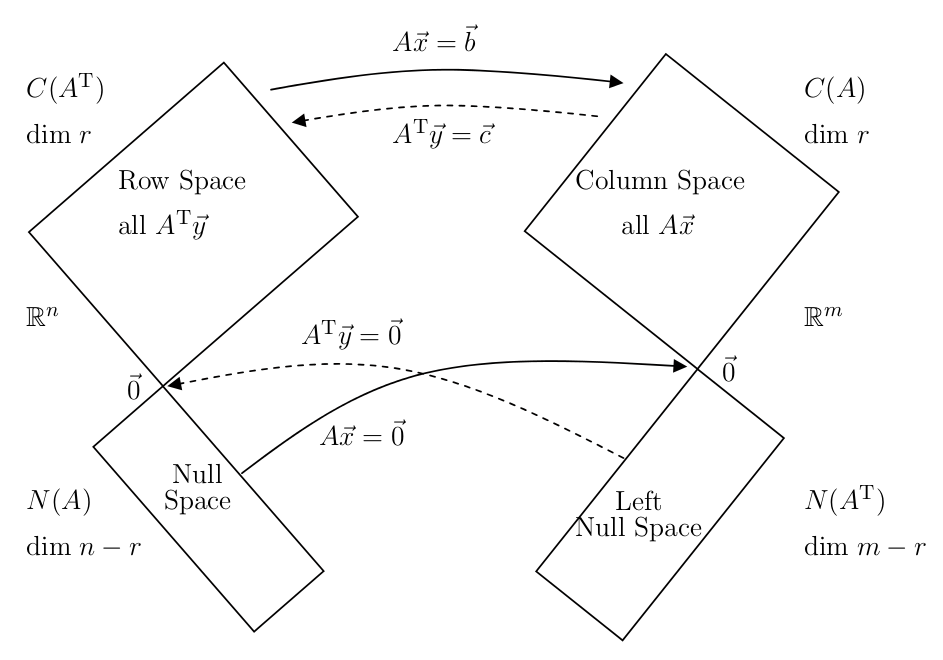
\includegraphics[width=14cm]{fund}
  \caption{Visualization of the Fundamental Theorem of Linear Algebra}
  \label{fig:fund}
\end{figure}
\hfill

Strang goes further in contextualizing the SVD factorization in the
above diagram (\cite{strang93}), by noting that the columns of the
matrices $V$ and $U$, actually contain the basis of these four
subspaces: 

\begin{itemize}
\item The orthogonal matrix $V$ contains a basis for the row space
  \C{\trans{A}} in the first $r$ columns, and a basis for the null
  space \N{A} in the last $n-r$ columns. We showed this already while
  proving \cref{thm:SVD2}. 
\item The orthogonal matrix $U$ contains a basis for the column space
  \C{A} in the first $r$ columns, and a basis for the left null
  space \N{\trans{A}} in the last $m-r$ columns. 
\end{itemize}
\hfill

The last observation makes the SVD factorization even more astonishing
and intriguing: not only it allows one to understand the true nature of
an arbitrary matrix $A$, by explicitly giving the two change of basis
that make $A$ a positive diagonal matrix $\Sigma$ (having just
compressions and expansions). Also, if we consider a basis as a 
representation of a vector space; then the matrices $V$ and $U$ of the
SVD factorization can be 
considered a representation of the four subspaces generated by that
particular matrix $A$. Putting together the three matrices as in $A =
U\Sigma\trans{V}$, gives the truly complete picture about the effects
of transformation $A$. 

